\chapter{Calibration}
\label{calib}
The shaper amplifiers used to process the detector signals provide only a rough gain adjustment.  Each of the 72 signals that are read out from the detector array must be calibrated using analysis software.  In addition, each detector has a timing signal associated with it which also needs to be calibrated.  
In all, 96 different signals need to be matched with one another.  The visualization and analysis of the data is carried out with the program ROOT, which is based on the programming language C++~\cite{Brun_1998}.  The method by which the data are calibrated takes the form of C++ macros which are used to generate functional fits to the data.  The calibration constants determined by the fits are stored in calibration files which are read in and applied during the sorting of the data.
\section{Position}
The measured position as formulated in Eq.~\ref{detector_X} assumes that the two position signals $X_\mathrm{far}$ and $X_\mathrm{near}$ are gain-matched.  This relation further assumes that the sum of the two position signals are in turn gain-matched to the measured energy $E$.  The latter consideration may be circumvented by use of Eq.~\ref{x_noE}. % of Eq.~\ref{detector_redund} .
% However, in order for the measured position to have physical relevance,the two position signals must be gain-matched. and corrected for ballistic deficit.
\subsection{Gain-matching}
In an un-calibrated detector, the following relation holds true.
\begin{equation}
a(E)=b(X_\mathrm{near})+c(X_\mathrm{far})
\label{eq:cal}
\end{equation}
The most fundamental level of calibration of the detector array is the determination of the constants $a$, $b$, and $c$ for each given detector.  The first step of this process is the relative, mutual calibration, or gain-matching, of the two position signals.  If the position signals are not gain matched, then the derived position is distorted.  In the case when the calculation of the position includes all three signals (Eq.~\ref{detector_X}), the uncalibrated position will be compressed by a factor of $(b+c)/2$.  If instead, only two signals are used to calculate the position (Eq.~\ref{detector_redund}), the uncalibrated position will be compressed \textit{and} skewed in a non-linear fashion.  Fig.~\ref{xfxn} shows the method of determining the constants $b$ and $c$, discussed below.
\begin{figure}%
\centering
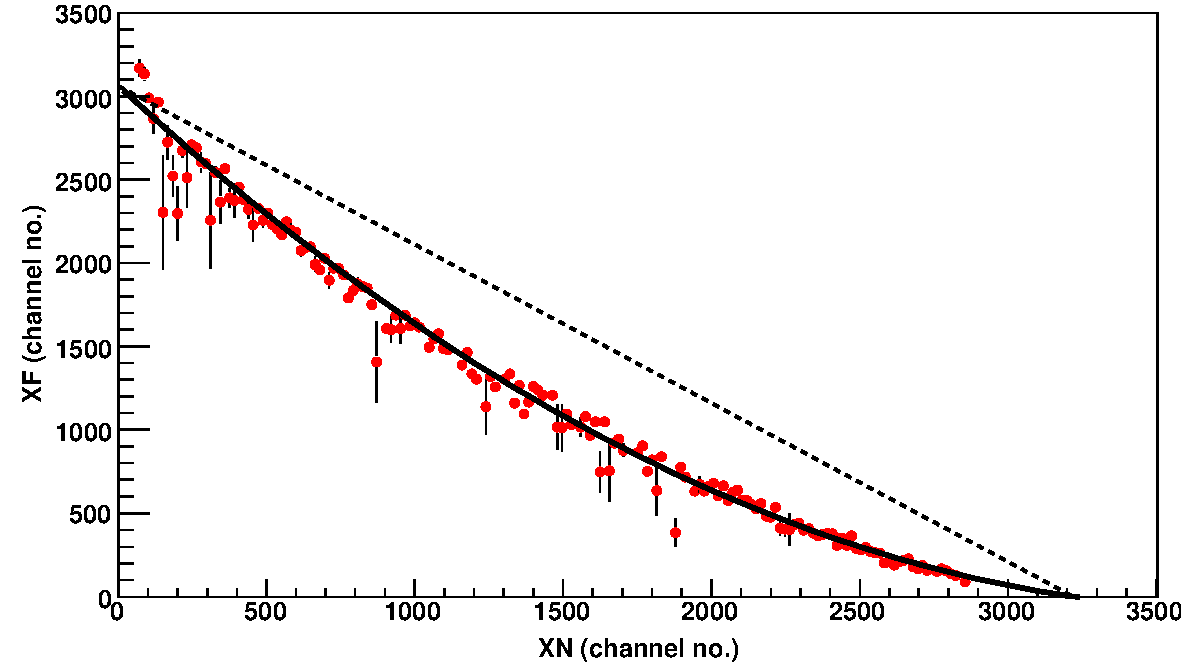
\includegraphics[width=\columnwidth]{cXFXN}%
\caption[Polynomial fit to a profile of a histogram of $X_\mathrm{far}$ vs. $X_\mathrm{near}$ for an individual detector]{Polynomial fit to a profile of a histogram of $X_\mathrm{far}$ vs. $X_\mathrm{near}$ for an individual detector.  In this example, the slope of the linear fit to the data (dashed line) is -0.951, meaning gain of the $X_\mathrm{far}$ signal is 95.1\% that of the $X_\mathrm{near}$ signal.}
\label{xfxn}%
\end{figure}

When properly gain-matched, the position signals are negatively correlated with a correlation coefficient of $-1$.  The first step of the calibration procedure is to measure the correlation coefficient of the uncalibrated detector.  This coefficient is determined by plotting the position signals in a two-dimensional histogram with one position as the abscissa and the other as the ordinate.  Measuring the slope of this histogram at a fixed energy gives the correlation coefficient.  This can be accomplished by measuring a spectrum of known, fixed energies, for instance the $\alpha$ particles from the decay of a  radioactive %$^{228}$Th
decay source.  

The fits shown in this chapter are made using the \texttt{TProfile} class available in ROOT~\cite{Brun_1998}.  A ``profile'' of a two-dimensional histogram (scatter-plot) is made by plotting the mean value of the $Y$-co\-or\-di\-nate at each $X$-po\-si\-tion.  Fig.~\ref{xfxn} shows the profile of the $X_\mathrm{far}$ vs. $X_\mathrm{near}$ histogram for a specific detector.  For a clear demonstration of this technique, an example has been selected where only one energy level is present, that of the 3.18\,MeV \label{typo1} $\alpha$-decay of $^{148}$Gd.  The figure shows a quadratic fit to the distribution of counts with an additional linear fit connecting the intercepts of the quadratic fit.  Higher-order polynomial terms do not improve the quality of the fit.  The relationship between the two detector signals is clearly not best described by a linear function.  This is due to an effect known as the ``ballistic deficit,'' discussed below.

Using this dual-fit technique, the slope of the linear fit provides the gain-matching coefficient very accurately.  The slope parameter is applied to the position signals such that the dispersion of either $X_\mathrm{far}$ or $X_\mathrm{near}$ is increased while the other is left un-scaled.  This corresponds to setting either $b$ or $c$ in Eq.\ref{eq:cal} equal to 1 and assigning the other a value $>1$.  For example, the slope of the linear fit in Fig.~\ref{xfxn} is $-0.951$, which means the $X_\mathrm{near}$ signal is unscaled ($b=1$) and the $X_\mathrm{far}$ signal is scaled by $1/0.951=1.051=c$.
 
\section{Noise Rejection}
Once the two position signals have been gain-matched, the energy signal can be gain-matched to the position signals by fitting a profile of a plot of $E$ vs. $(X_\mathrm{far} + X_\mathrm{near})$.  As was the case with the gain-matching of the positions signals, this step of the calibration is based on a linear fit of the above-mentioned plot.  Fig.~\ref{fig_esum}(a) shows such a plot after the gain-matching parameter has been applied.  It is interesting to note most of the points lie along a sharply-defined locus corresponding to $E=(X_\mathrm{far} + X_\mathrm{near})$.  This pronounced correlation between all three detector signals is accomplished simply by gain-matching all three signals---no higher-order correction have been applied.  However, not all of the points exhibit proper correlation.  The loci of points in the region indicated by the arrow in Fig.~\ref{fig_esum}(a) do not lie along the same line.

Fig.~\ref{fig_esum}(b) shows a projection of Fig.~\ref{fig_esum}(a) along the line $E=(X_\mathrm{far} + X_\mathrm{near})$.  From the area under the peaks, 91.5\% of the points lie along the line $E=(X_\mathrm{far} + X_\mathrm{near})$.  The remaining 8.5\% of the points are spurious.  The width of the main peak corresponds to the intrinsic detector resolution.  This peak has been aligned with zero using a new calibration constant $d$, which is applied as follows $E-(X_\mathrm{far} + X_\mathrm{near})+d$.  Aligning the $E-(X_\mathrm{far} + X_\mathrm{near})$ spectra this way allows the entire array to be gated with a single parameter.    Fig.~\ref{fig_esum}(c) shows a plot of $E$ vs. $X$ which includes all points.  The spurious points form a ridge at the edge of the detector, indicated by the arrow. Fig.~\ref{fig_esum}(d) shows a plot of $E$ vs. $X$ for the same data set which has been gated on Fig.~\ref{fig_esum}(b) to exclude points outside of the range $\left|E-(X_\mathrm{far} + X_\mathrm{near})\right|<30$.  Comparing Fig.~\ref{fig_esum}(c) to Fig.~\ref{fig_esum}(d) shows that the points along the edge of the detector have been eliminated.
\begin{figure*}%
\centering
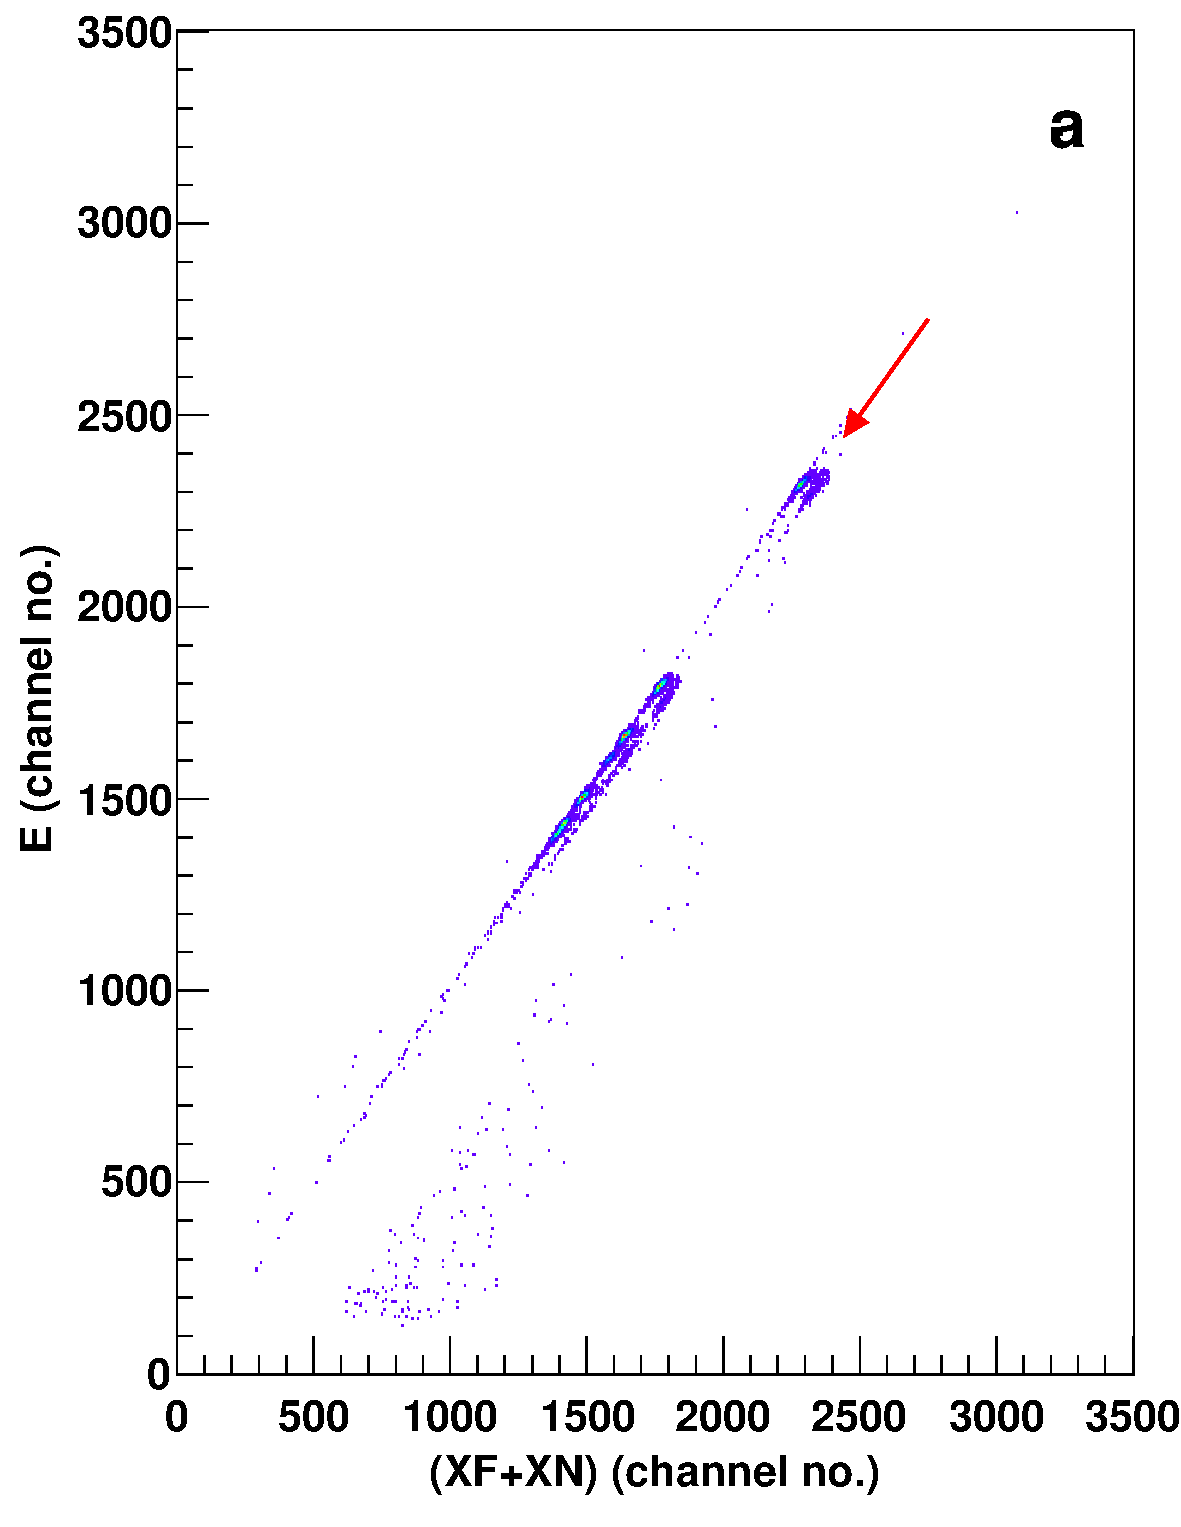
\includegraphics[width=0.45\textwidth,height=0.4\textheight,keepaspectratio]{cESum}~
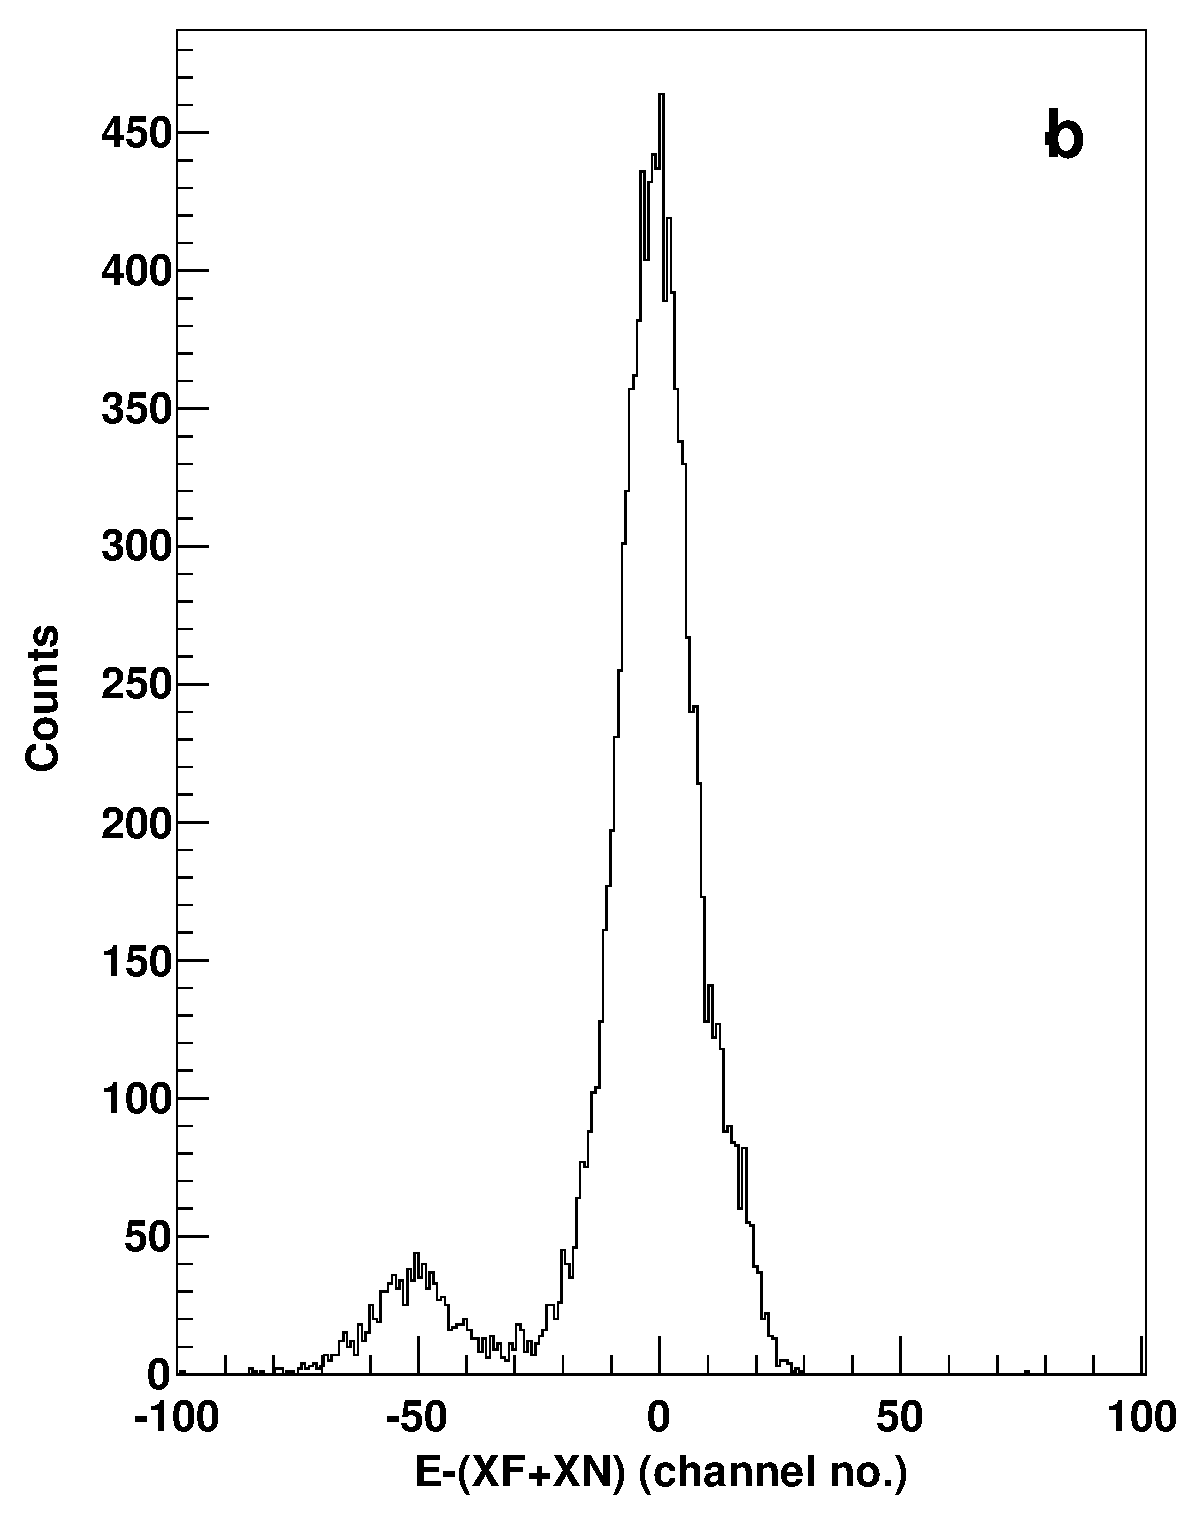
\includegraphics[width=0.45\textwidth,height=0.4\textheight,keepaspectratio]{cESum_pjy}\\
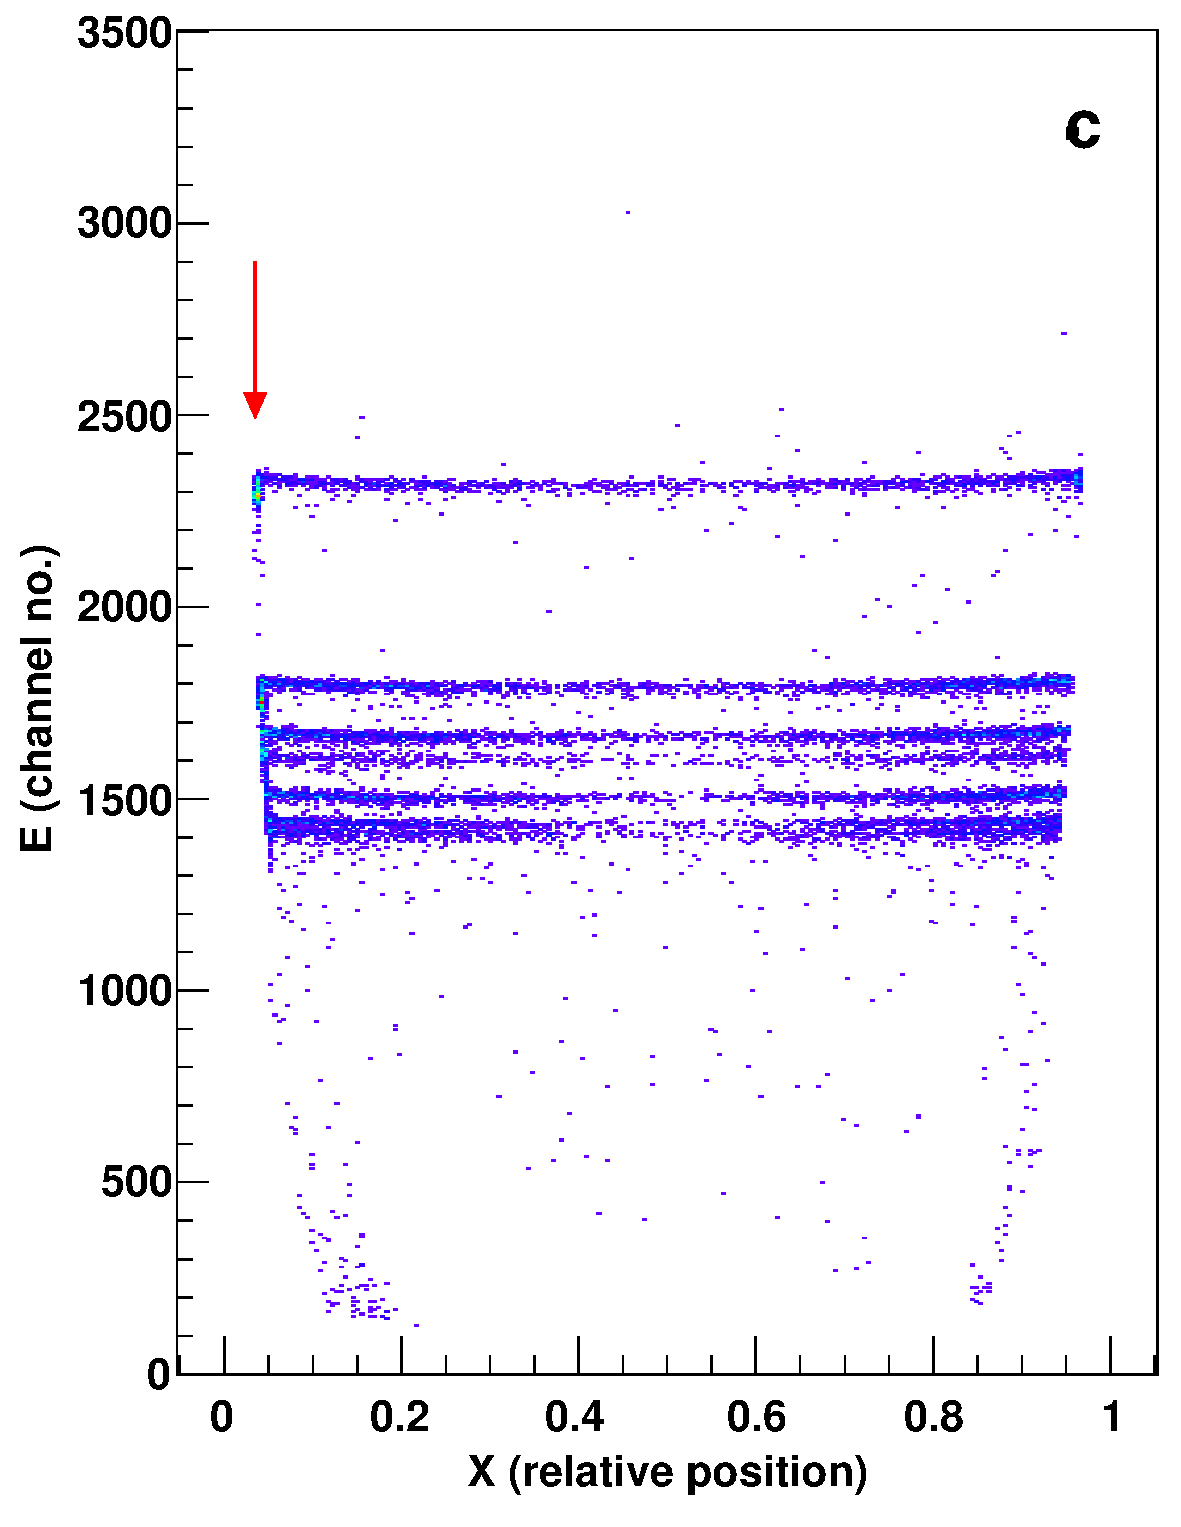
\includegraphics[width=0.45\textwidth,height=0.4\textheight,keepaspectratio]{cEX_nosum}~
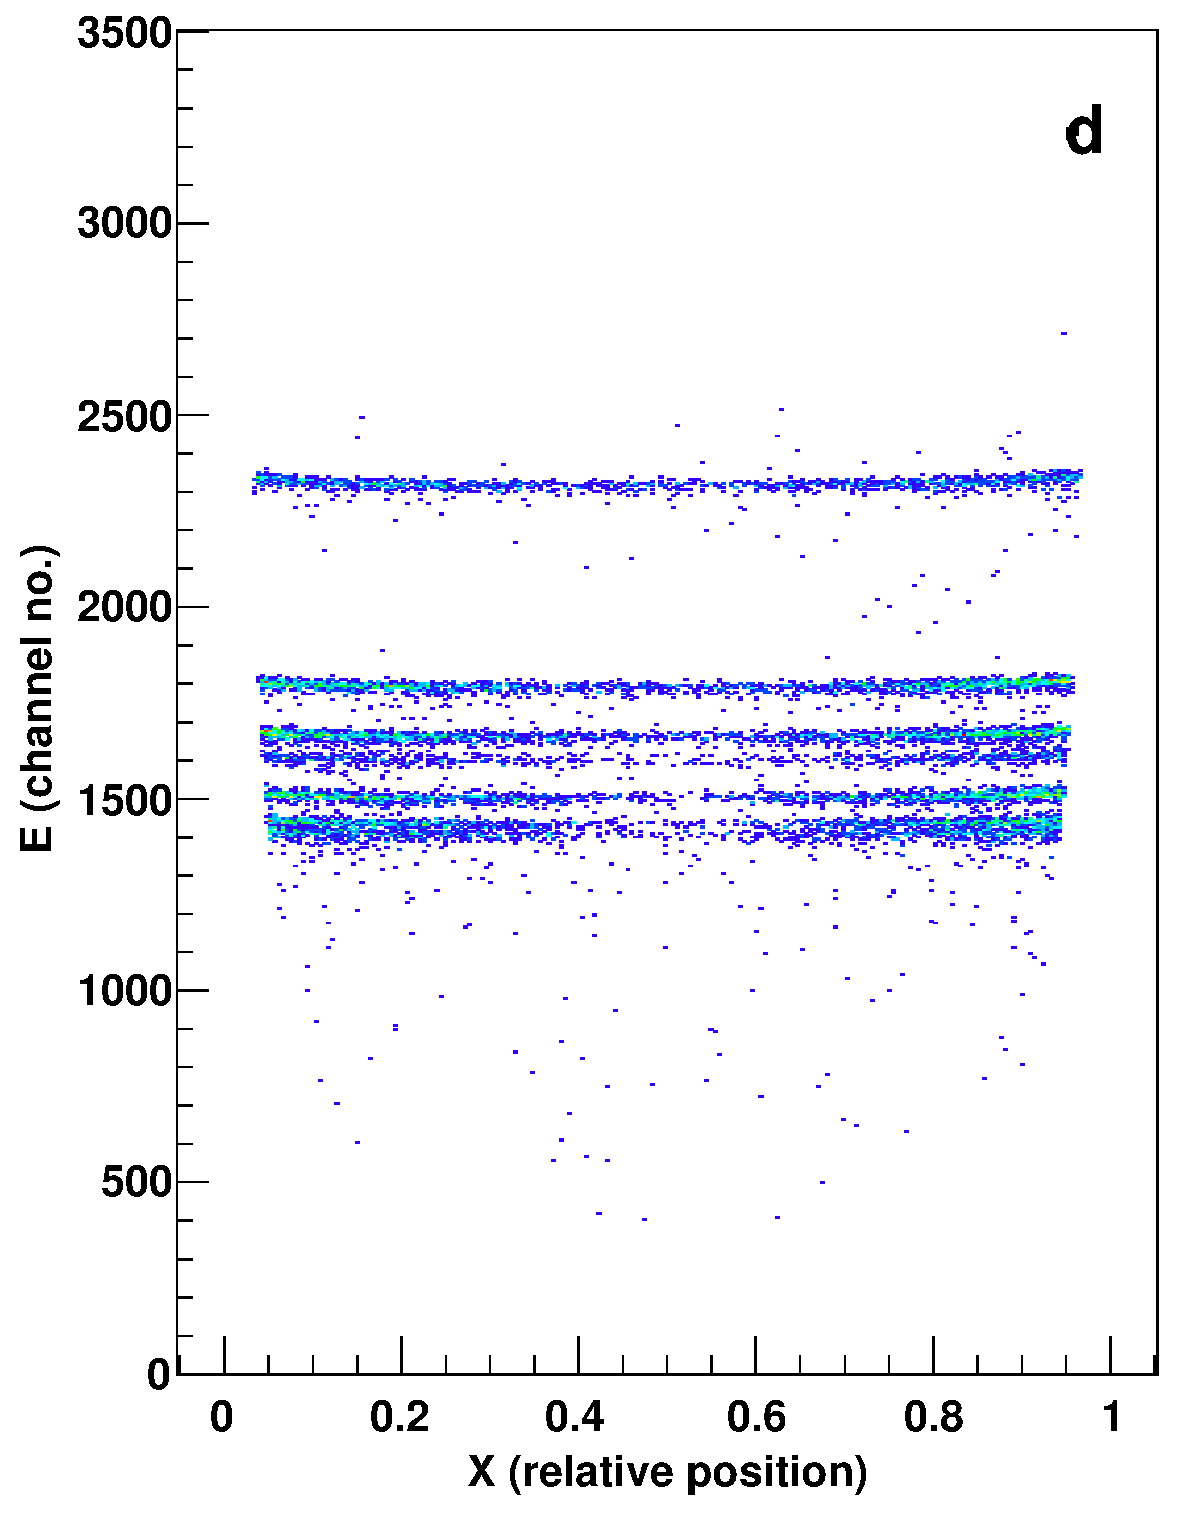
\includegraphics[width=0.45\textwidth,height=0.4\textheight,keepaspectratio]{cEX_sum}
\caption[Method of rejection spurious counts by gating $E-(X_\mathrm{far} + X_\mathrm{near})$]{Method of rejection spurious counts by gating $E-(X_\mathrm{far} + X_\mathrm{near})$. (a) Plot of $E$ vs. $(X_\mathrm{far} + X_\mathrm{near})$ for an individual detector.  The loci of counts that do not lie on the line $E=(X_\mathrm{far} + X_\mathrm{near})$, indicated by the arrow, are spurious.  (b) Projection of panel (a) along the line $E=(X_\mathrm{far} + X_\mathrm{near})$. The peak corresponding to the ``good'' events have been aligned with zero.  The width of the peak is equal to the intrinsic resolution of the detector. (c) $E$ vs. $X$ spectrum with no points excluded.  The loci of points in the region indicated by the arrow correspond to the smaller peak in panel (c). (d) $E$ vs. $X$ spectrum requiring $E=(X_\mathrm{far} + X_\mathrm{near})$ which no longer has pathological points at the detector edges.}%
\label{fig_esum}%
\end{figure*}

\section{Energy}
The energy of the detector is calibrated by measuring a known energy spectrum.  The peaks in the spectrum are found using the \texttt{TSpectrum} class within ROOT~\cite{Morhac_2000}.  In the example shown in Fig.~\ref{peakfit}, 7 known peaks are identified in the $\alpha$-decay chain of $^{228}$Th.  The \texttt{TSpectrum} class provides the channel numbers of the peaks, which are then mapped to their corresponding energy values with a linear fit.  In this example, the ADC channel number is converted to energy in MeV with the relation $E=(E_0+1386)/523$, where $E_0$ is the uncalibrated energy.  To preserve the relation $E=(X_\mathrm{far} + X_\mathrm{near})$, these same calibration constants can be applied to the position signals as $X=(X_0+f)/g$, where $f$ and $g$ are the offset and slope, respectively, of the linear fit.

\begin{figure}%
\centering
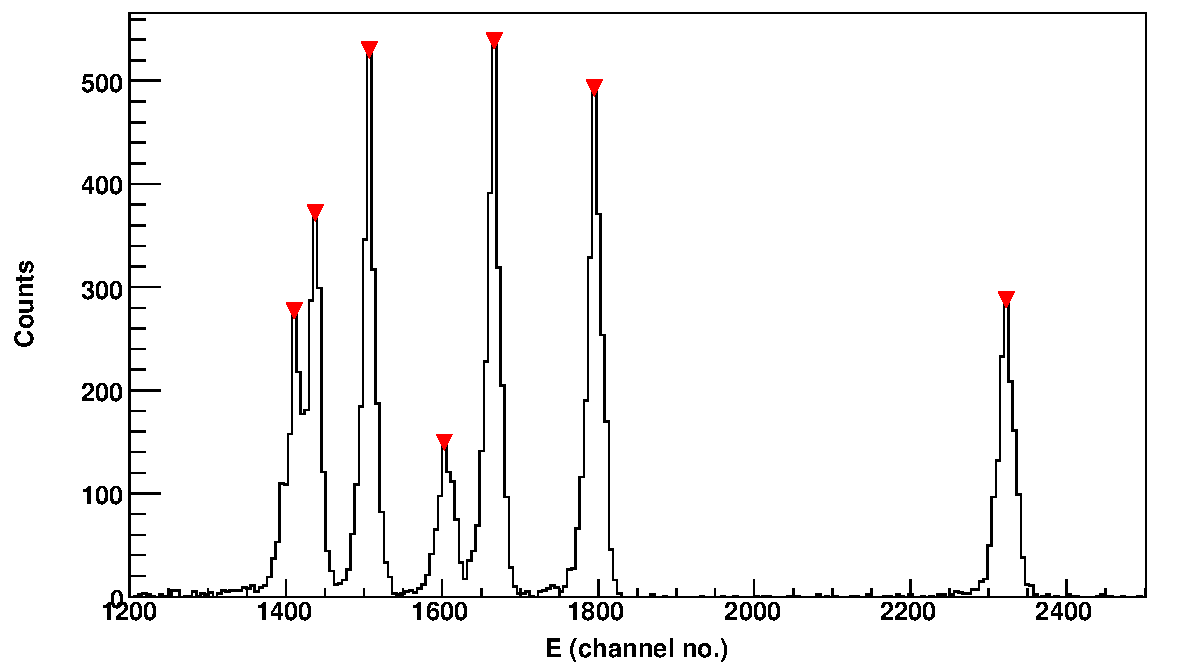
\includegraphics[width=\columnwidth,height=0.5\textheight,keepaspectratio]{cEpeaks}%
\caption[Uncalibrated $\alpha$-decay energy spectrum for an individual detector]{Uncalibrated $\alpha$-decay energy spectrum for an individual detector.   Peaks from the $^{228}$Th $\alpha$-decay chain identified using \texttt{TSpectrum}~\cite{Morhac_2000}.}%
\label{peakfit}%
\end{figure}

In all, the basic calibration of the three individual detector signals can be accounted for with five calibration constants per detector: two parameters to gain-match the position and energy signals; one parameter to align the projection of $E-(X_\textrm{far}+X_\textrm{near})$; and two parameters to calibrate the energy.  In practice, these calibration constants are stored in a single calibration file, 24-lines long with 5 elements per line (plus an indexing element).  The varying subtleties of each detector (such as measured background, noise, and resolution) preclude the automated generation of these constants and mandate that this process be carried out manually.  Such a calibration file can be generated for a set of data in a few hours.

\section{Ballistic Deficit}
Given a finite pulse-shaping time constant in a shaping amplifier, a slower rise time of a preamplifier signal will  lead to an effective attenuation of the resulting shaped-pulse signals.  In other words, the signals with slower rise times are measured to have a lower energy.  The amount by which the amplitude of the shaped signal is reduced from what would be attained with an infinite shaping time is known as the ballistic deficit~\cite{Knoll_1979}.  If the rise time of the preamplifier signal is the same for all signals, this effect is uniform for all pulses and can be accounted for with the linear energy calibration technique discussed above.  However, if there is a variation in rise time of the preamplifier signals, the amplitude of the shaped energy signal will be dependent on rise time.

\subsection{Formalism}
\citet{Kalbitzer_1967} show that the charge collection at the energy contact of a PSD is described by the equation 
\begin{equation}
\begin{split}
Q_E(x,t)=(-2Q_0/\pi)\sum_{n=1}^\infty n^{-1}\sin[n\pi (x/L)]\times \left[1-\cos(n\pi)\right]\left[1-\textrm{e}^{-n^2\pi^2\frac{t}{(RC)}}\right]
\end{split}
\label{eq:charge}
\end{equation}
where $Q_0$ is the charge of the incident particle; $R$ is the resistance of the implanted resistive strip; and $C$ is the capacitance of the detector junction. Fig.~\ref{rise_times} shows a plot of this equation, specifically $Q/Q_0$ vs. $\pi^2t/(RC)$, for a variety of detection positions.  Eq.~\ref{eq:charge} depends explicitly on $x/L$ and this dependence is shown clearly in Fig.~\ref{rise_times}.  For example, the charge collection time at the energy contact to go from 10\%$Q_0$ to 90\%$Q_0$ is 1.6$\times$ longer at $x/L=0.5$ compared with $x/L=0.1$.  This position dependence of the charge collection time translates to a position dependence of the rise time of the signal from the preamplifier.  The rise times of the position signals can be described in an equivalent fashion.

\begin{figure}%
\centering
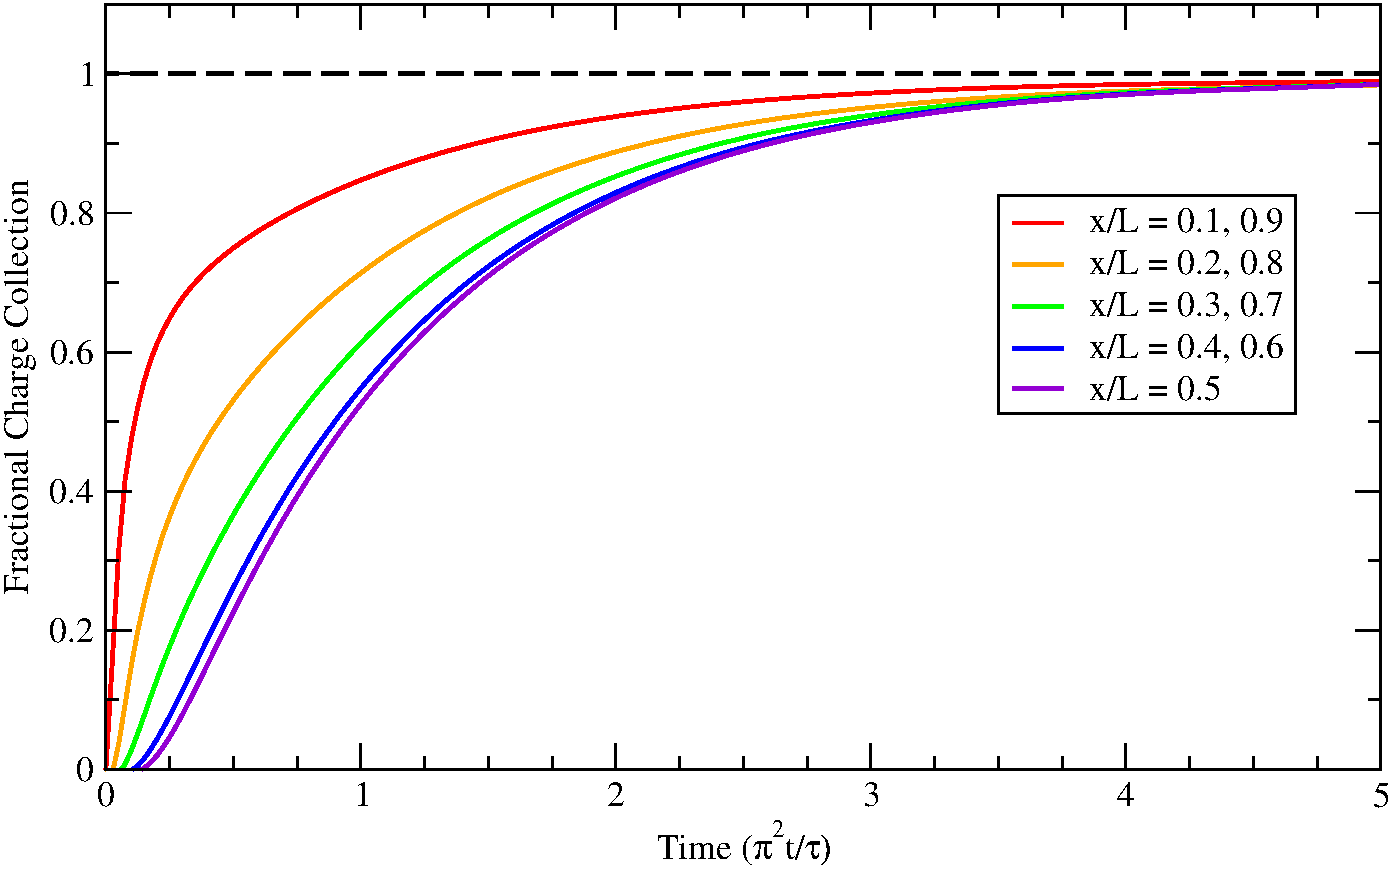
\includegraphics[height=0.5\textheight,width=\columnwidth,keepaspectratio]{rise_times}%
\caption[Charge collection times for a typical PSD calculated at a variety of detection positions]{Charge collection times for a typical PSD calculated at a variety of detection positions.  The charge collection times---and therefore the preamplifier signal rise times---are greatest at the center of the detector.  Adapted from Ref.~\cite[Fig.~4]{Kalbitzer_1967}}%
\label{rise_times}%
\end{figure}
The effect of the ballistic deficit can be clearly seen in Figs.~\ref{xfxn} and \ref{energy_plot} by deviation between the measured data and the dashed lines corresponding the no ballistic deficit.  The detector characteristics shown in these plots are very similar to those shown in Ref.~\cite[Fig.~2]{Doehring_1968}, which presents computational modeling of ballistic deficit.  To first order, the effect of ballistic deficit can be ignored.  For example, close examination of Figs.~\ref{cezg_350} and \ref{double}, as reported in \citet{Lighthall_2010}, reveals that this effect has not been corrected for.  However, neglecting this effect reduces the effective detector energy resolution.  If an energy level is averaged over the length of a detector element, the position-dependence of the energy will lead to a decrease in the resolution of the energy.  In addition, given the relationship in Eq.~\ref{eq:cal}, the position signals also exhibit ballistic deficit.  The result is that the measured position is artificially compressed about the central region of the detector. 

\subsection{Compensation}
There are a number of approaches for correcting for the ballistic deficit causing the position dependence of the energy.  Perhaps the most straight-forward approach begins with an even-order polynomial fit of the $X$-projection of the energy.  Fig.~\ref{energy_plot} shows such a fit for an individual detector.  With a fit in hand, the ballistic deficit can be corrected using the equation  

\begin{equation}
E=E_0-\sum_{i=1}^{2n} a_i x^i
\label{ecal}
\end{equation}
where $E_0$ is the uncorrected energy.  Given Eq.~\ref{eq:cal}, once a detector has been gain-matched, the same fit may be used to correct the ballistic deficit in both the position signals and the energy.  The position signals are scaled by a factor of $E/E_0$.  However, it is important to note that the effect of ballistic deficit is also energy-dependent.  Although this feature is not represented in the simplified expression of Eq.~\ref{eq:charge}, it is empirically true.  Therefore caution must be used when applying this technique; it is suitable for optimizing a particular energy level, but a full correction must utilize energy dependence.

\begin{figure}%
\centering
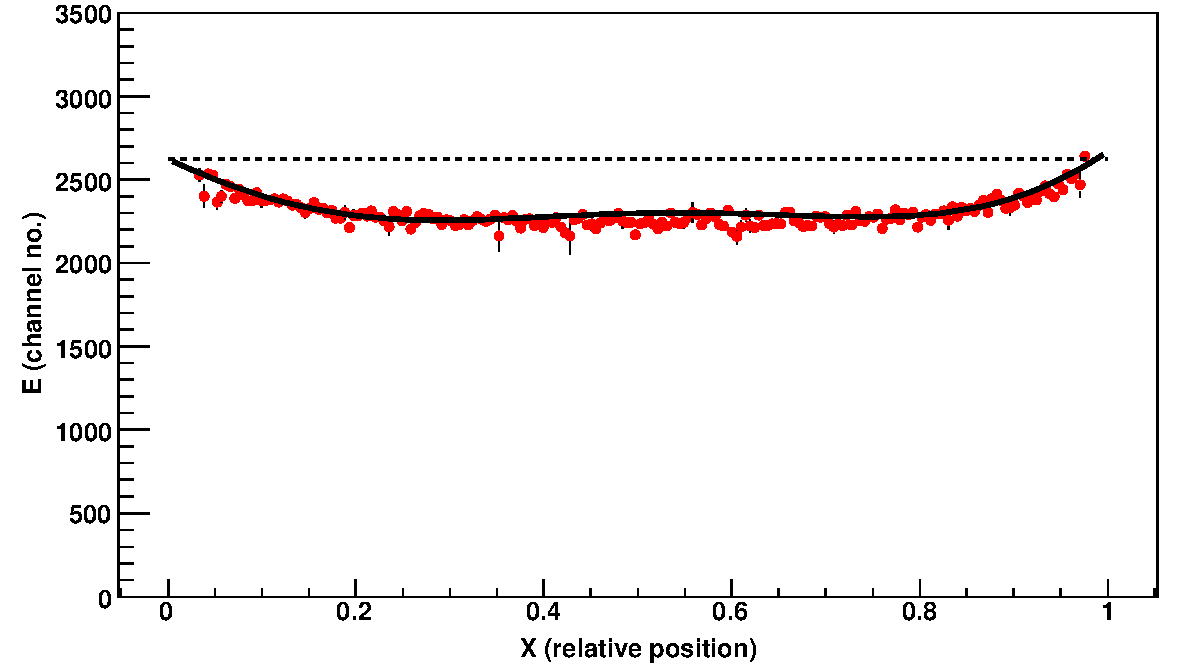
\includegraphics[width=\columnwidth]{cEX}%
\caption[Polynomial fit to the projection of a $E$ vs. $X$ histogram for a detector exhibiting ballistic deficit]{Polynomial fit to the projection of a $E$ vs. $X$ histogram for a detector exhibiting ballistic deficit.  The dashed line corresponds to an ideal detector with no ballistic deficit.  Compare to Fig.~\ref{xfxn}. }

\label{energy_plot}%
\end{figure}

\section{Time-of-flight} 
Two energy-dependent effects contribute to the timing signal being skewed.  The first arises from kinematics; shallow orbits intercept the array at earlier times; this effect is sharply energy-dependent and decreases the measured flight times on the order of about 2\,ns.  However, the contribution of this effect is generally less than the time resolution of the detector at the energy which it occurs.  The second effect is related to the ballistic deficit and is on the order of the time resolution at low energy.

Fig.~\ref{time_plot} shows an uncalibrated energy versus time plot for a typical detector.  The structural details of this histogram are effectively identical to those reported in Ref.~\cite[Fig.~9]{Bennett_1992}, which discusses the timing response of PSDs in general.  The apparent skewing towards longer flight times at low energy arises from the use of a constant fraction discriminator to produce the timing signals.   The timing signals produced by a CFD are susceptible to rise time walk.  As discussed in the previous section, the pulse shapes (rise times) are position dependent in a PSD.  

As can be seen in Fig.~\ref{time_plot}, the time walk feature only occurs at lower energy; thus a fit is needed that is only applied at low energy.  The solution employed in calibrating the HELIOS data uses piecewise quadratic fit to the low-energy timing structure.  The fit is generated by an iterating macro which takes as its input the rough coordinates of an individual timing peak in $E$-$T$ space.  For example, in Fig.~\ref{time_plot} the single-orbit proton peak is roughly located in a box 400--1000 channels in $T$ and 400-3000 channels in $E$.  The macro takes the profile of this box and fits the profile with a quadratic function.  Then macro then iterates the endpoint of the fit until the critical point of the quadratic function corresponds to the endpoint of the fit.  The result is shown in Fig.~\ref{time_fit}.


Once the piecewise fit has been calculated, the time walk is corrected with the following 
\begin{equation}
\forall T_0<\left(\frac{-p_1}{2P_2}\right)\qquad T=T_0-p_2\times \left(E+ \frac{p_1}{2 p_2}\right)^2
\label{eq:time}
\end{equation}
where $p_n$ is the $x^n$ coefficients of the quadratic fit and $T_0$ is the uncorrected time.  The resulting time spectrum is independent of energy, to within a possible residual linear offset.  

Finally, the timing response of the detectors is also position dependent.  The form of which is nearly identical to ballistic deficit and can be corrected for using the same method described above for correcting the position-dependence of the energy.  Fig.~\ref{time_cal} shows the time versus position spectra for an individual detector before and after calibration.  In the uncalibrated spectrum, the timing response is slower in the center of the detector (corresponding to lower channel numbers). In the calibrated spectrum, an even-order polynomial fit has been used to remove the position dependence and the channel number has been calibrated to time in ns.

\begin{figure}[hb]
\centering
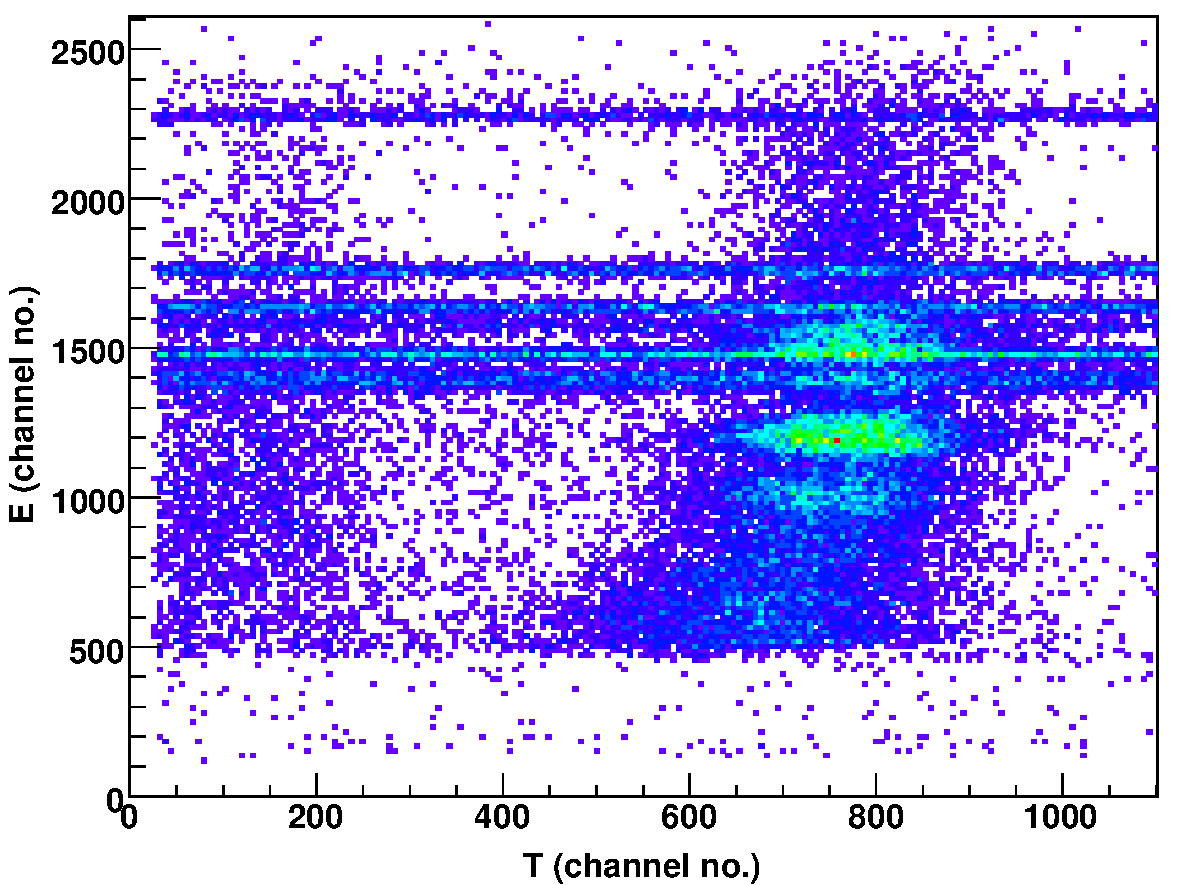
\includegraphics[width=\columnwidth]{cET}%
\caption[Uncalibrated time spectrum for a typical detector showing time walk]{Uncalibrated timing spectrum for a typical detector showing characteristic time walk.  Increasing times correspond to decreasing channel number with a dispersion of approximately $-18$\,ns per channel number.  The prominent locus near channel 700 corresponds to single-orbit protons and the locus near channel 100 corresponds to double orbits.}%
\label{time_plot}%
\end{figure}

\begin{figure}[p]
\centering
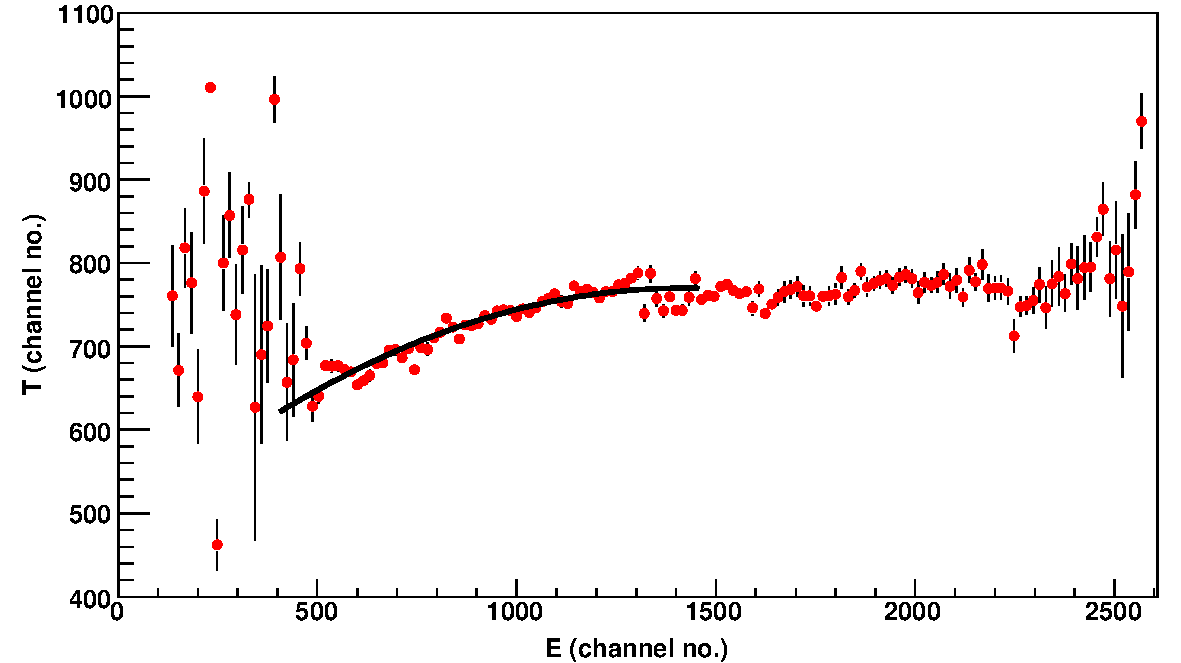
\includegraphics[width=\columnwidth]{cET_pfy}
\caption[Piecewise quadratic fit to a time profile to correct time walk]{Piecewise quadratic fit to a time profile to correct time walk.  The $Y$-Profile of the histogram in Fig.\ref{time_plot} is plotted.  The endpoint of the fit (channel 1422) corresponds to the critical point of the fit.  The distribution beyond the critical point ($E>1422$) is roughly constant, \textit{i.e.}, linear.}%
\label{time_fit}%
\end{figure}

\begin{figure}[p]
\centering
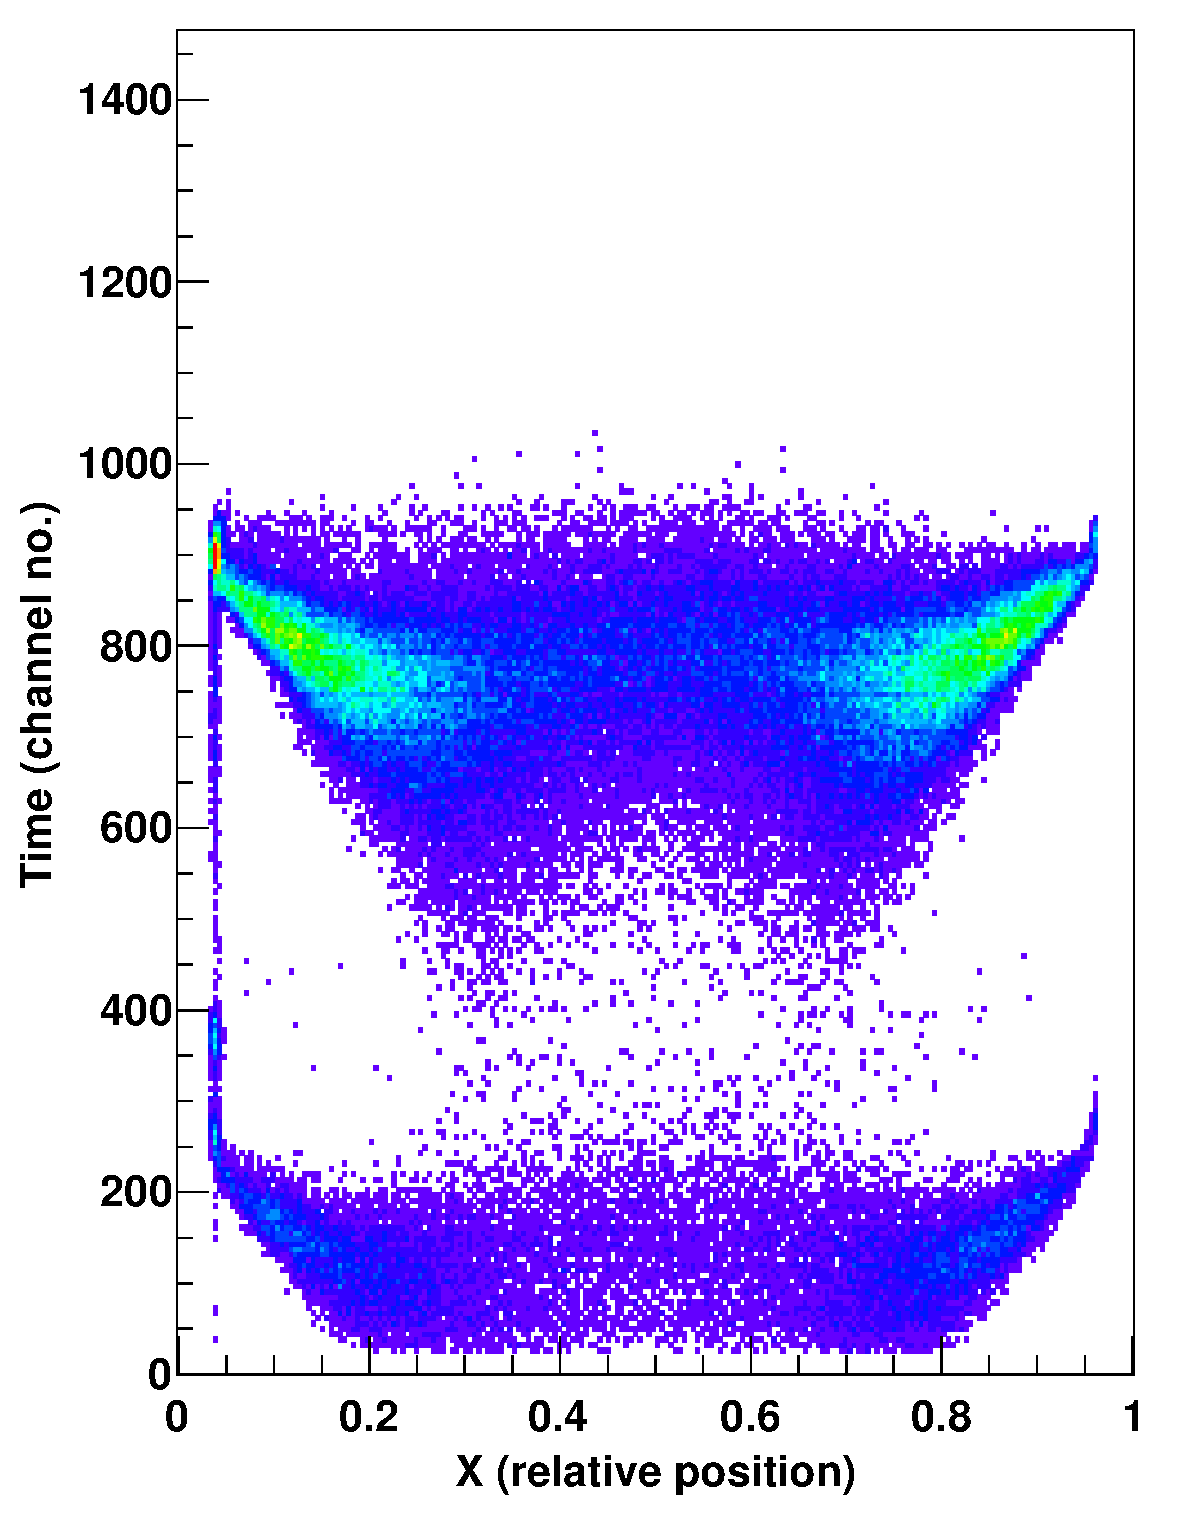
\includegraphics[width=0.45\textwidth,height=0.45\textheight,keepaspectratio]{cTnocal}~
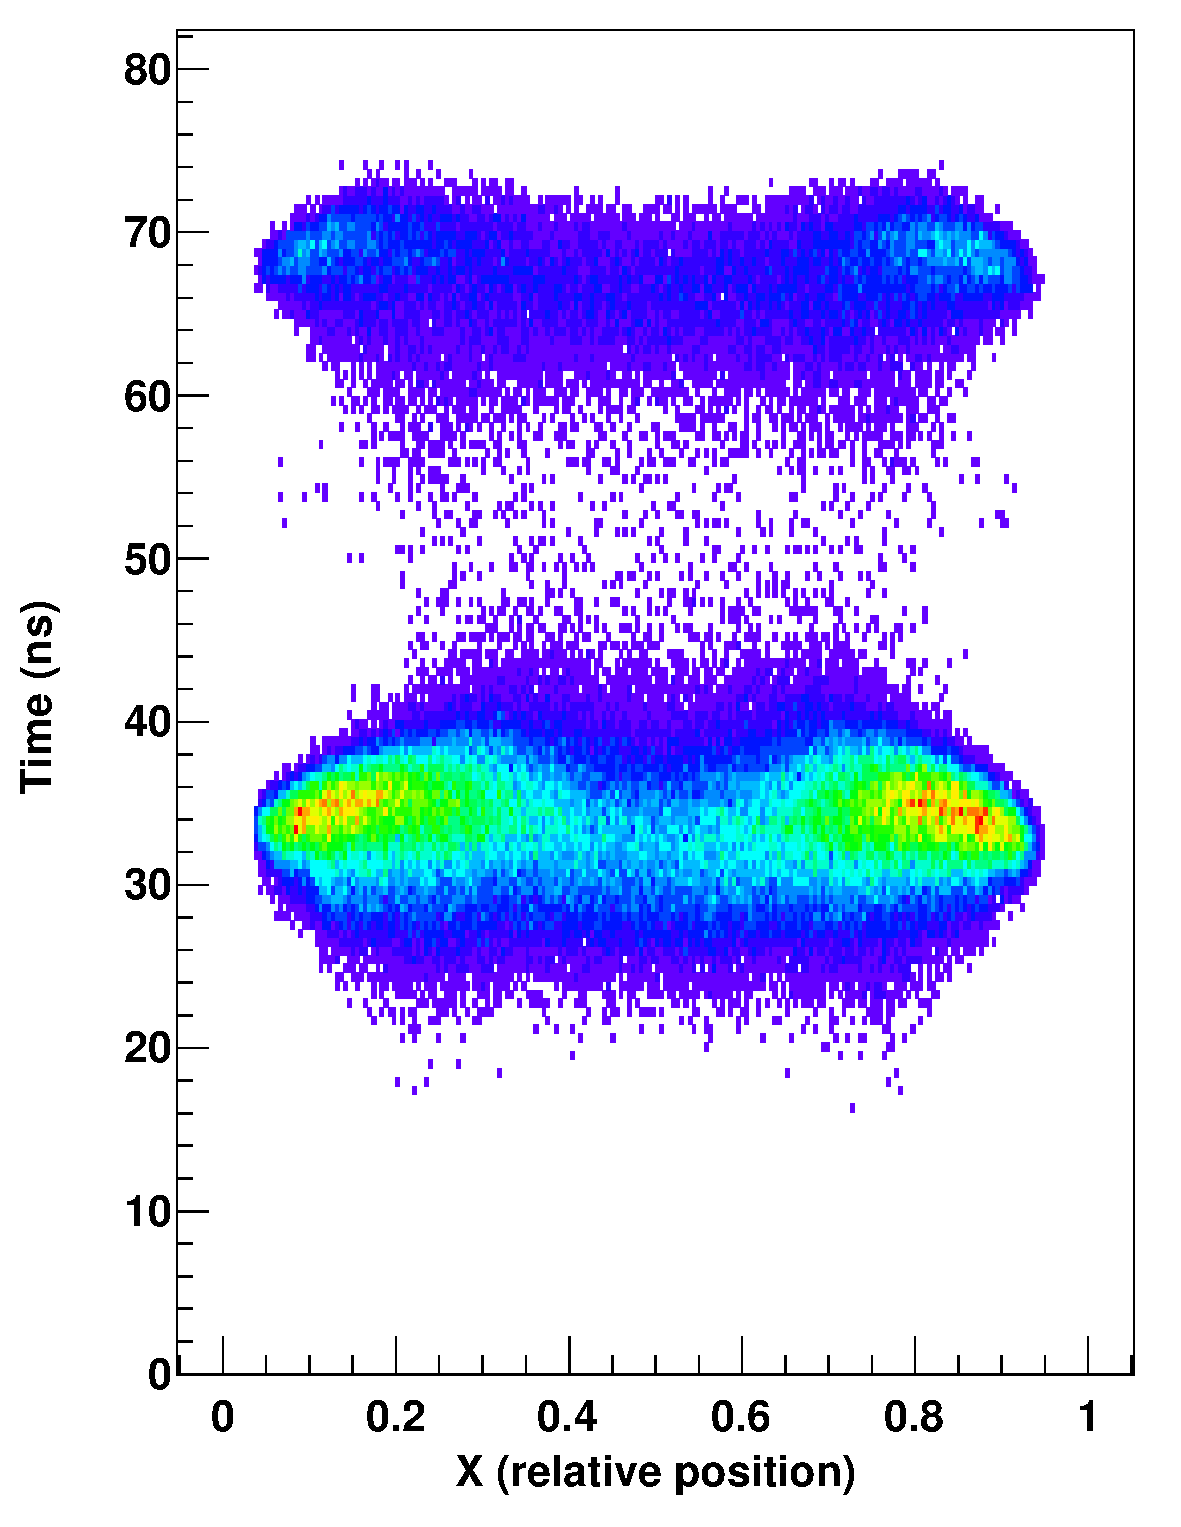
\includegraphics[width=0.45\textwidth,height=0.45\textheight,keepaspectratio]{cTcal}\\
\caption[Time vs. position spectrum before (left) and after (right) calibration]{Time vs. Position spectrum before (left) and after (right) calibration for an individual detector.  An even-order polynomial fit has been used to correct the position dependence.  The range of the $y$-axis in both panels corresponds to 82\,ns, but is reversed on the left due to the dispersion of $-18$\,ns per channel.}%
\label{time_cal}%
\end{figure}